\documentclass[../main.tex]{subfiles}
\graphicspath{
    {"../img/"}
    {"img/"}
}

\begin{document}
     \begin{figure}[h]
        \centering
        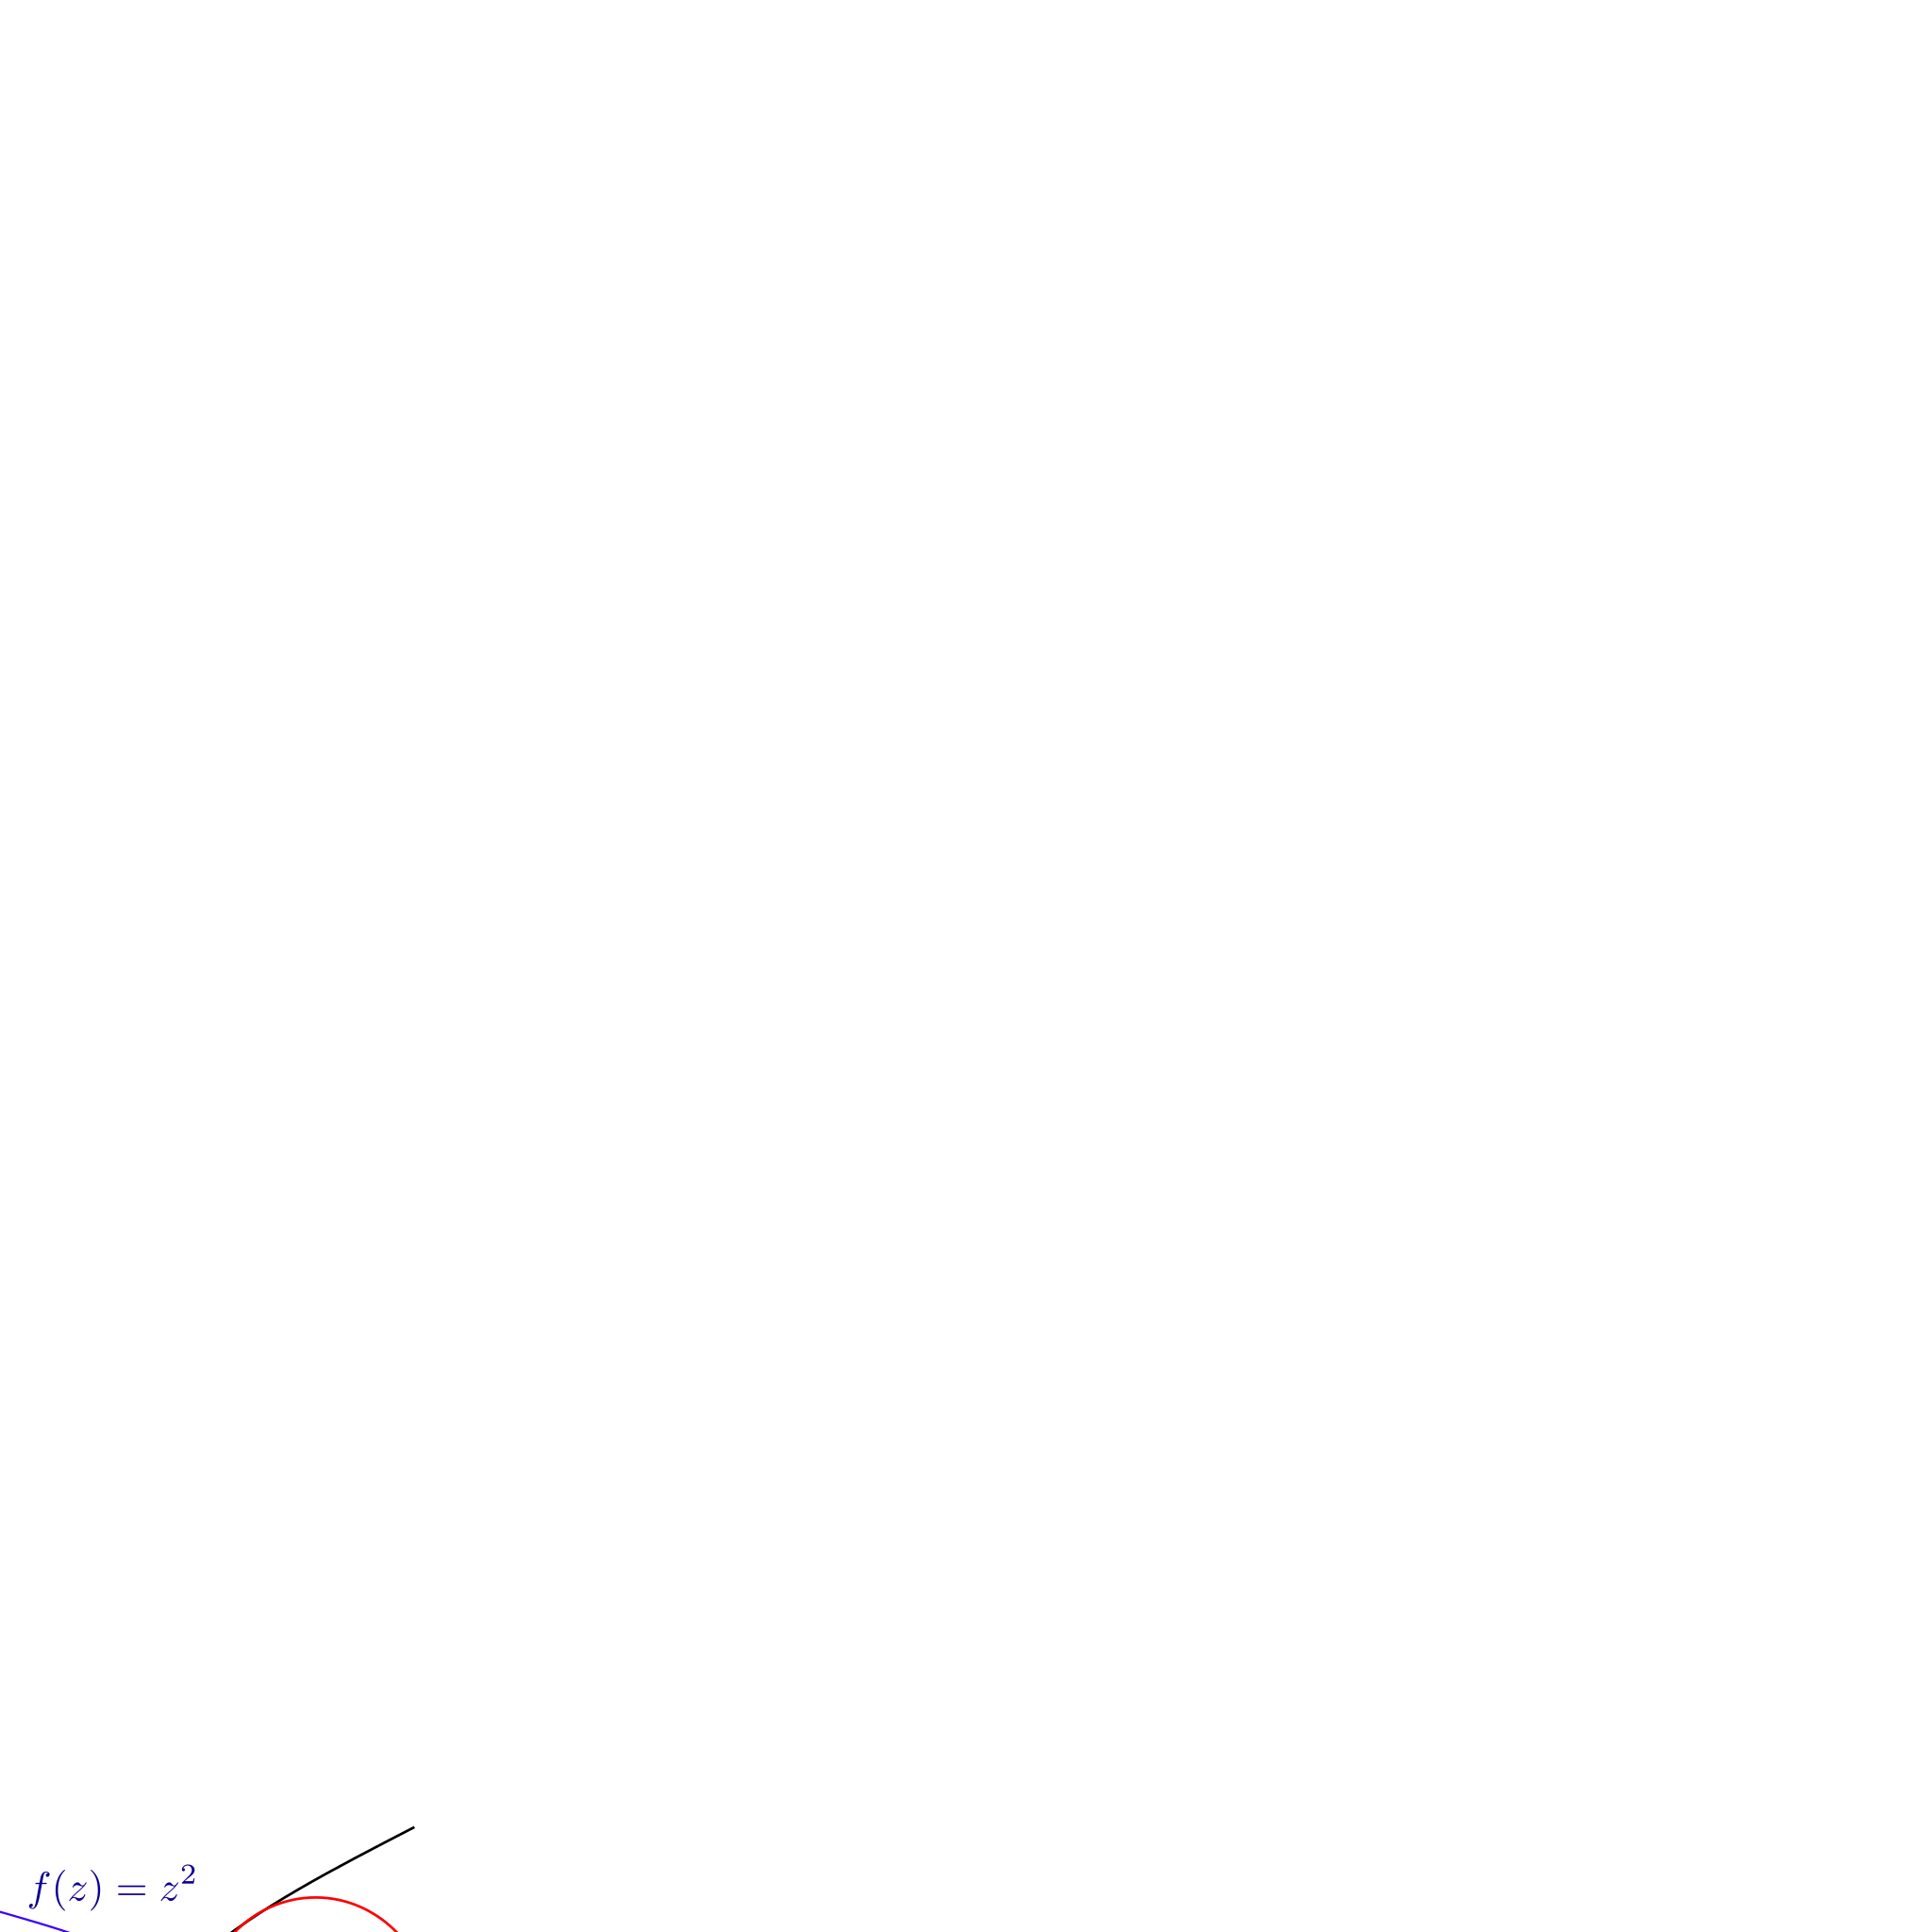
\includegraphics[width=0.8\textwidth]{w19-1}
        \caption{}
        \label{fig:w19-1}
    \end{figure}
    \subsubsection{Sprawdzamy jak zmienia się promień krzywizny przy transformacji $f(z)$} (rys \ref{fig:w19-1}).
    \[
        \frac{1}{s} = \frac{Im(\ddot{z}\overline{\dot{z}})}{\left| \dot{z} \right| ^3}
    .\]
\[
    \frac{1}{\tilde s} = \frac{Im\left(\left(\frac{d^2}{dt^2}\left( z(t) \right) ^2 \overline{\frac{d}{dt}|z(t)|}\right)\right)}{\left| \frac{d}{dt}\left( z(t) \right) ^2 \right| ^3}
.\]
\[
    \tilde z (t) = \left( z(t) \right) ^2
.\]
\[
    \left( \dot{\tilde z}(t) \right)' = \left( 2\left(z(t)\left( \dot{z}(t) \right) \right) \right)' = 2 \dot{z}(t) \dot{z}(t) + 2z(t) \ddot{z}(t)
.\]
\[
    \left( \overline{\tilde z} \right)' = \left( \tilde z(t) \tilde z(t) \right)' = 2 \overline{z}(t) \overline{\dot{z}}(t)
.\]
\[
    \ddot{\tilde z} \cdot \overline{\dot{\tilde z}} = \left( 2(\dot{z}(t))^2 + 2z(t)\ddot{z}(t)\right)\left( 2\overline{z}(t)\overline{\dot{z}}(t) \right) = 4\overline{z}(t) \left| \dot{z} \right| ^2 \dot{z}(t) + 4\left| z(t) \right| ^2 \overline{\dot{z}}(t) \cdot \ddot{z}(t)
.\]
Ale
\[
    \frac{Im( \tilde \ddot{z} \overline{\dot{\tilde z}})}{\left| \dot{\tilde z}(t) \right|^3 } = \frac{Im\left| 4\overline{z}(t) \right| (\dot{z}(t))^2 \cdot \dot{z}(t)}{8\left| z(t) \right| ^3 \left| \dot{z}(t) \right| ^3} + \frac{Im(4 \left| z(t) \right| ^2 \overline{\dot{z}}(t) \ddot{z}(t))}{8\left| z(t) \right| ^3 \left| z(t) \right| ^3}
.\]
Zatem
\[
    \frac{1}{\tilde s} = \frac{1}{2\left| z(t) \right| }\left( \frac{Im\left( \overline{z}(t)\dot{z}(t) \right) }{\left| z(t) \right| ^2 \left| z(t) \right|} + \frac{1}{s} \right)
.\]
Ale
\[
    \overline{z}(t) \dot{z}(t) = \left( x(t) - iy(t) \right) \left( \dot{x}(t) + i\dot{y}(t) \right) = x\dot{x} + y\dot{y} + i\left( x\dot{y} - y\dot{x} \right)
.\]
\[
    Im\left( \overline{z}(t)\dot{z}(t) \right) = x\dot{y} - y\dot{x} = \begin{bmatrix} x&\dot{x}\\ y&\dot{y} \end{bmatrix} = \left| \overline{z}(t) \right|\cdot \left| \dot{z}(t) \right| \sin(\sphericalangle \dot{z}(t), \overline{z}(t))
.\]
\[
    \frac{1}{\tilde s} = \frac{1}{2\left| z(t) \right| }\left( \frac{\left| z(t) \right| \left| \dot{z}(t) \right| }{\left| z(t) \right| ^2 \cdot \left| \dot{z}(t) \right| } \sin(\sphericalangle(\dot{z}, \overline{z})) + \frac{1}{s}\right)
.\]
\[
    \frac{1}{\tilde s} = \frac{1}{2 \left| z(t) \right| } \left( \frac{\sin(\sphericalangle(\dot{z}, \overline{z}))}{\left| z(t) \right| } + \frac{1}{s} \right)
.\]
\subsubsection{Już prawie twierdzenie Kasner-Arnold}
Rozważmy ruch na $\mathbb{R}^2$, pod wpływem siły $F = -r$, czyli na $\mathbb{C}$
 \[
     \ddot{z}(t) = -z(t),\text{ gdzie }\left( m = 1, k = 1 \right)
.\]
\begin{figure}[h]
    \centering
    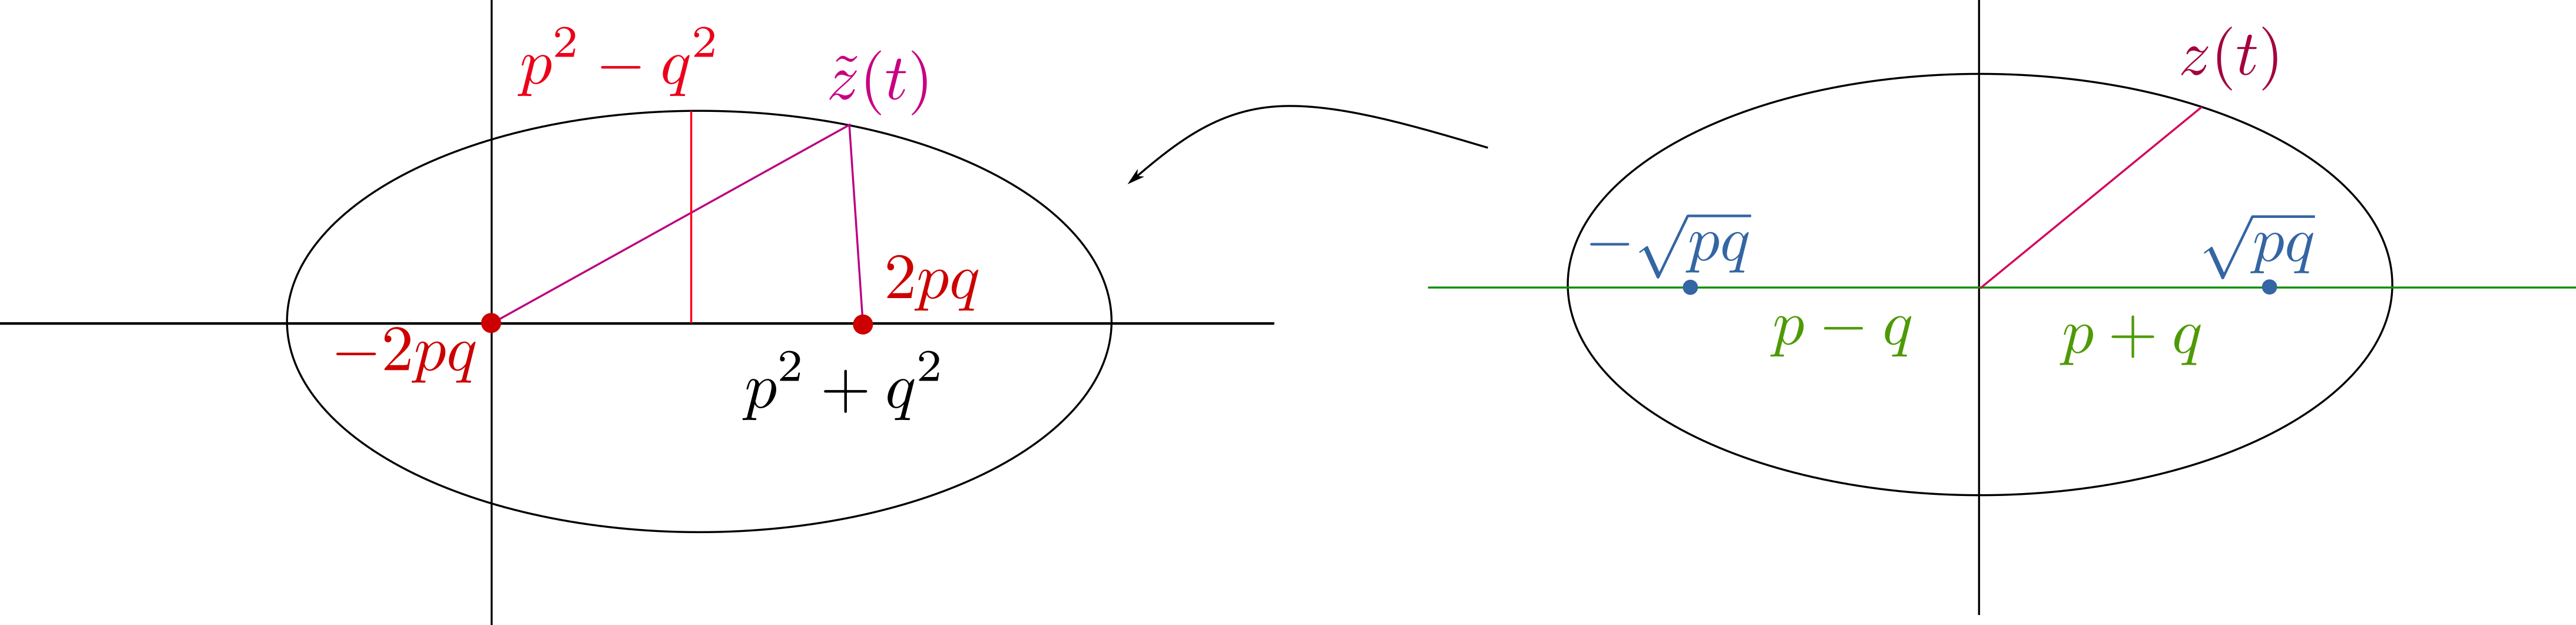
\includegraphics[width=0.8\textwidth]{w19-2}
    \caption{przed i po}
    \label{fig:w19-2}
\end{figure}
Trajektoria wygląda tak:
\[
    z(t) = pe^{it} + qe^{-it} = \left( p+q \right) \cos(t) + i(p-q)\sin(t)
.\]
\[
    \left( x(t), y(t) \right) = \left((p+q)\cos(t), (p-q)\sin(t)\right)
.\]
Jak rozpoznać siłę typu $F = -\frac{1}{r^2}$ od $F = -r$? Trajektoria wychodzi taka sama, ale dla tej drugiej siła jest zaczepiona w środku elipsy. Co się stanie jak przepuścimy tę elipsę przez $f(z) = z^2$? Dostaniemy
\[
    \tilde z(t) = \left( p e^{it} + qe^{-it} \right) ^2 = p^2 e^{2it} + 2pq + q^2e^{-2it} = \left( p^2 + q^2 \right) \cos(2t) + 2pq + i(p^2 - q^2)\sin(2t)
\]
taką przesuniętą elipsę jak na rys. \ref{fig:w19-2}
\begin{pytanie}
    \begin{figure}[h]
        \centering
        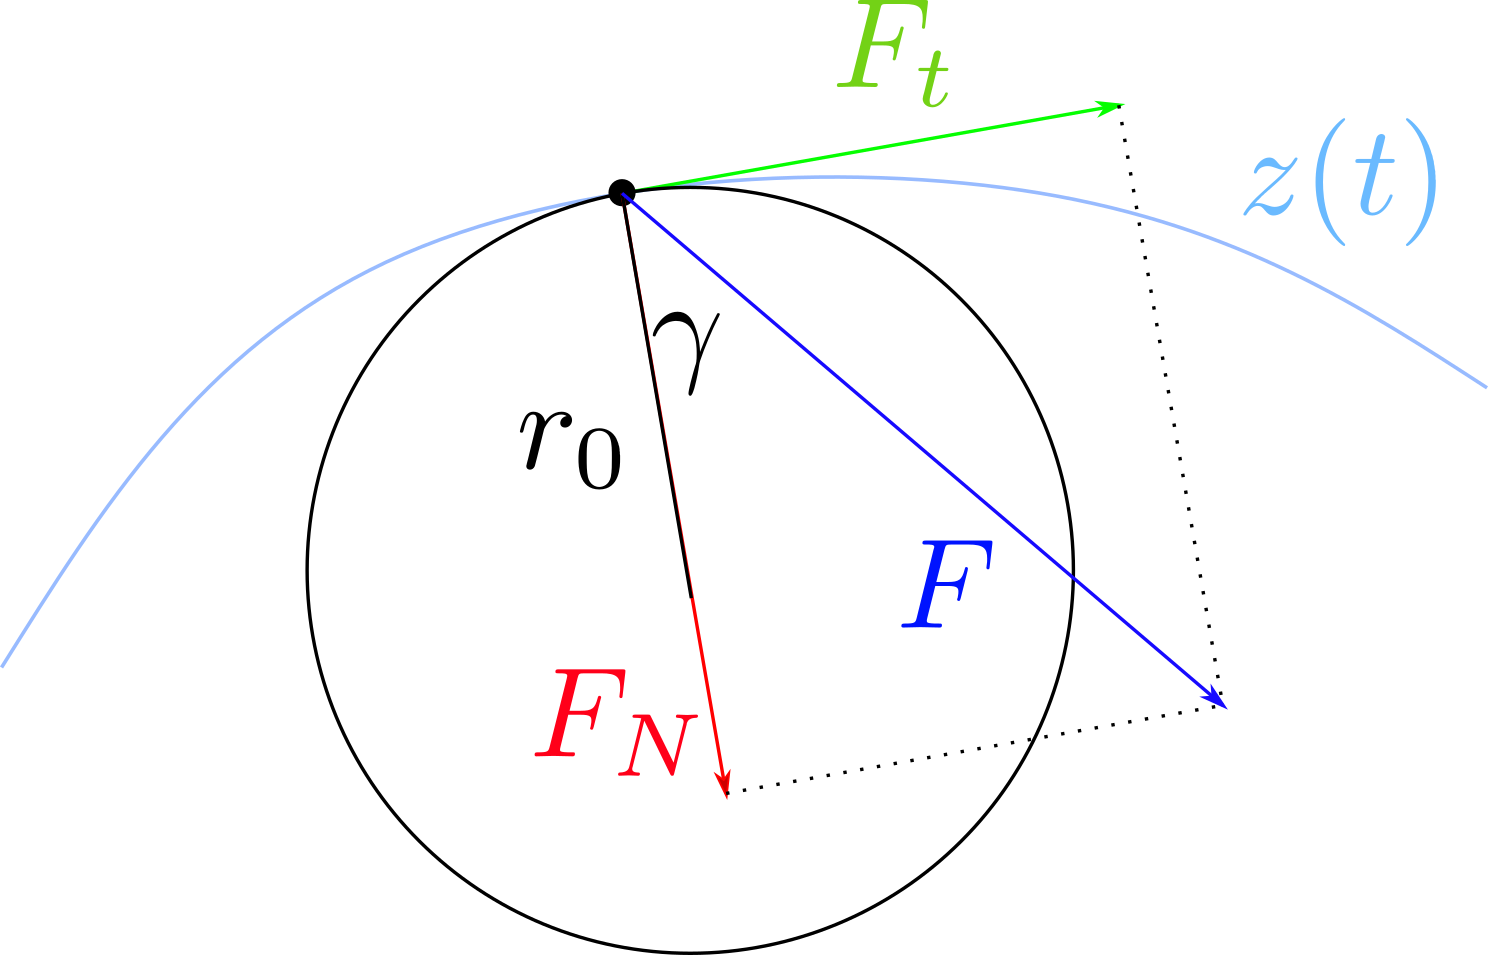
\includegraphics[width=0.3\textwidth]{w19-3}
        \caption{}
        \label{fig:w19-3}
    \end{figure}
    Jeżeli $F = -r$, To jaka jest $\tilde F$? (sytuacja jak na rys. \ref{fig:w19-3})
\end{pytanie}
        $\cos\gamma = \frac{F_N}{F},\quad F = \frac{F_N}{\cos\gamma}$, ale $F_N = \frac{v^2(t)}{r_0}$. My wiemy, że czasami zachowany jest moment pędu
        \[
            \overline{r} \times \overline{v}(t) = r \cdot v \sin(\sphericalangle r, v) = r v \cos\gamma = const = A
        .\]
    Czyli
    \[
    v = \frac{A}{r \cos\gamma}
    .\]
\[
    F = \frac{F_N}{\cos\gamma} = \frac{1}{r_0}\frac{A^2}{r^2(\cos\gamma)^3}
.\]
I dostaliśmy taki związek. Dla ruchu po okręgu $\gamma = 0$,  $r = r_0$ i wtedy
\[
    F = \frac{1}{r^3}A^2 = \frac{1}{r^3}(r v)^2 = \frac{v^2}{r}
    .\]
Znowu spróbujemy przepuścić taki ruch przez $f(z) = z^2$. Przypuszczamy, że będą takie zmiany:
\begin{align*}
    A &\sim \tilde A\\
    r &\sim \tilde r\\
    r_0 &\sim \tilde r_0\\
    \gamma &\sim \gamma \quad \text{(bo $f(z)$ - koforemna)}\\
    v &\sim \tilde v\\
    F &\sim \tilde F
.\end{align*}
Ale
\[
    F = \frac{A^2}{r_0}\frac{1}{r^2}\frac{1}{\left( \cos\gamma \right) ^3}
.\]
Zatem
\[
    \tilde F = \frac{1}{\tilde r_0}\frac{(\tilde A)^2}{\tilde r^2}\cdot \frac{1}{\left( \cos\gamma \right) ^3}
.\]
$A$ i $\tilde A$ się nie przejmujemy, ale za to $r_0$ już tak
\[
    \frac{1}{\tilde r_0} = \frac{1}{2 r}\left( \frac{1}{r_0} + \frac{\overset{\sin(\sphericalangle(\dot{z}, \overline{z}))}{\cos\gamma}}{r} \right)
.\]
Z tego co wcześniej napisaliśmy, mamy
\[
    \frac{1}{r_0} = \frac{F}{(A)^2}r^2(\cos\gamma)^3
.\]
Wtedy
\[
    \frac{1}{\tilde r_0} = \frac{1}{2r}\left( \frac{\cos\gamma}{r} + \frac{F}{(A)^2}r^2(\cos\gamma)^3 \right)
.\]
\[
    \frac{1}{\tilde r_0} = \frac{1}{r}\frac{(\cos\gamma)^3}{(A)^2}r\left( \frac{(A)^2}{2r^2(\cos\gamma)^2} + \frac{Fr}{2} \right)
.\]
\[
    \frac{1}{\tilde r_0} = \frac{(\cos\gamma)^3}{(A)^2}\left( \frac{1}{2}v^2 + \frac{Fr}{2} \right)
.\]
Zauważmy, że gdy $F \sim r$, to
 \[
     \frac{1}{2}v^2 + \frac{1}{2}r^2 = E
.\]
(Energia całkowita ruchu po elipsie, przed przepuszczeniem przez $f(z) = z^2$ )
\[
    \frac{1}{\tilde r_0} = \frac{(\cos\gamma)^3}{\left( A \right) ^2} \cdot E
.\]
Zatem podstawiając do wcześniej wyliczonego $\tilde F$ mamy
\[
    \tilde F = \frac{(\cos\gamma)^3 E}{(A)^2}\cdot \frac{(\tilde A)^2}{\tilde r^2}\frac{1}{(\cos\gamma)^3} = \left( \frac{\tilde A}{A} \right) ^2 \frac{E}{\tilde r^2} = \frac{const}{\tilde r^2}
.\]
To jest dowód Kasnera - Arnolda w przypadku $f(z) = z^2$. Siły grawitacji i te $\sim r$ okazują się być w jakiejś "dualności" względem $z^2$.
\begin{tw}
    (Kasner-Arnold)\\
    Jeżeli $F_1\sim r^A$, a $F_2\sim r^{\tilde A}$ i
    \[
        \left( A+3 \right)(\tilde A + 3) = 4
    \]
    i $m = \frac{A+3}{2}$, to transformacja $f(z) = z^m$ przeprowadza ruch (trajektorię i cały ten posag) pod wpływem siły $F_1$ w ruch pod wpływem siły $F_2$.
\end{tw}
\begin{przyklad}
    sprężyna - $A = 1$, $\tilde A = -2$, $m = \frac{1+3}{2} = 2$
    \[
        (1+3)(-2+3) = 4
    .\]
Wtedy nasz $f$ wynosi $f(z) = z^2$.
\end{przyklad}

\end{document}
